\documentclass{minimal}

\usepackage[paperwidth=20cm,paperheight=10cm,margin=1cm]{geometry}

\usepackage[utf8]{inputenc}
\usepackage[T1]{fontenc}
\usepackage[american]{babel}

\usepackage{tikz}
\usetikzlibrary{automata,arrows}

\newcommand{\anobs}[1][\mathtt{k}]{\mathcal{O}_{#1}}
\newcommand{\baseobs}{\anobs[\mkern-1mu\mathit{Base}]}
\newcommand{\ebrobs}{\anobs[\mkern-1mu\mathit{EBR}]}
\newcommand{\translab}[2]{\ensuremath{#1,\,#2}}
\newcommand{\translabbr}[2]{\ensuremath{#1},\\\ensuremath{#2}}
\newcommand{\anadr}{a}
\newcommand{\athread}{t}
\newcommand{\threadvar}{z_{t}}
\newcommand{\adrvar}{z_a}
\newcommand{\evt}[2]{#1(#2)}
\newcommand{\enter}{\mathtt{enter}}
\newcommand{\enterof}[1]{\enter\:#1}
\newcommand{\exit}{\mathtt{exit}}
\newcommand{\exitof}[1]{\exit\:#1}
\newcommand{\free}{\mathtt{free}}
\newcommand{\freeof}[1]{\free(#1)}
\newcommand{\retire}{\mathtt{retire}}
\newcommand{\leaveQ}{\mathtt{leaveQ}}
\newcommand{\enterQ}{\mathtt{enterQ}}

\newcounter{ObserverStateCounter}
\newcommand{\mkstatename}[1]{\stepcounter{ObserverStateCounter}${\arabic{ObserverStateCounter}}$}


\begin{document}
	\centering

	The SMR automaton specifying Epoch-Based Reclamation (EBR) is defined by $\baseobs\times\ebrobs$.
	\vspace{1cm}

	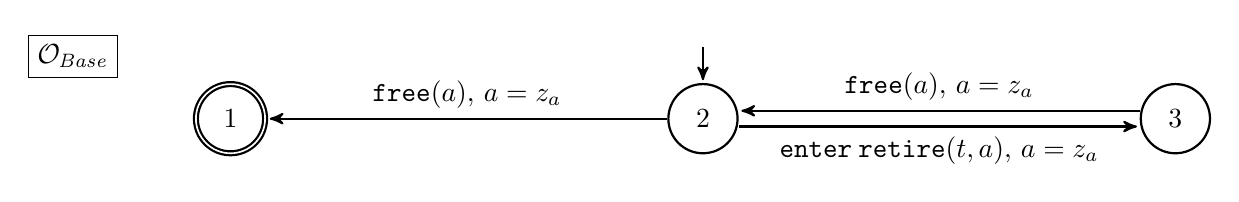
\begin{tikzpicture}[->,>=stealth',shorten >=1pt,auto,node distance=6cm,thick,initial text={}]
		\node [xshift=-2.0cm,yshift=.79cm,draw,thin] {$\baseobs$};
		\node[accepting,state]      (C)               {\mkstatename{obs:base:final}};
		\node[initial above, state] (A) [right of=C]  {\mkstatename{obs:base:init}};
		\node[state]                (B) [right of=A]  {\mkstatename{obs:base:retired}};
		\path
			([yshift=1mm]B.west) edge node [above]{\translab{\freeof{\anadr}}{\anadr=\adrvar}} ([yshift=1mm]A.east)
			([yshift=-1mm]A.east) edge node [below]{\translab{\evt{\enterof{\retire}}{\athread,\anadr}}{\anadr=\adrvar}} ([yshift=-1mm]B.west)
			(A) edge node [above]{\translab{\freeof{\anadr}}{\anadr=\adrvar}} (C)
			;
	\end{tikzpicture}
	\vspace{1cm}

	\begin{tikzpicture}[->,>=stealth',shorten >=1pt,auto,node distance=5cm,thick,initial text={}]
		\node [xshift=-0.4cm,yshift=1.2cm,draw,thin] {$\ebrobs$};
		\node[initial,state]    (A)              {\mkstatename{obs:ebr:init}};
		% \node[state]            (B) [right of=A,xshift=1cm] {\mkstatename{obs:ebr:invoked}};
		\node[state]            (E) [right of=A] {\mkstatename{obs:ebr:protected}};
		\node[state]            (C) [right of=E] {\mkstatename{obs:ebr:retired}};
		\node[accepting,state]  (D) [right of=C] {\mkstatename{obs:ebr:final}};
		\coordinate             [below of=A, yshift=+3.5cm]  (X)  {};
		\coordinate             [below of=E, yshift=+3.5cm]  (Y)  {};
		\coordinate             [below of=B, yshift=+3.5cm]  (Z)  {};
		\path
			(A) edge node[align=center] {\translabbr{\evt{\exitof{\leaveQ}}{\athread}}{\athread=\threadvar}} (E)
			(E) edge node[align=center] {\translabbr{\evt{\enterof{\retire}}{\athread,\anadr}}{\anadr=\adrvar}} (C)
			(C) edge node[align=center] {\translabbr{\freeof{\anadr}}{\anadr=\adrvar}} (D)
			(Y) edge[-,shorten >=0pt] node[text width=2.7cm] {
					\translab{\evt{\enterQ}{\athread}}{\athread=\threadvar}
					% \newline\translab{\evt{\unguard}{\athread,\anint}}{\athread=\threadvar}
				} ([xshift=-1mm]X)
			(E) edge[-,shorten >=0pt] ([yshift=1.5mm]Y.north)
			(C.south west) edge[-,shorten >=0pt] (Y)
			([xshift=-1mm]X) edge ([xshift=-1mm]A.south)
			([yshift=1.5mm]Y) edge[-,shorten >=0pt] ([xshift=1mm,yshift=1.5mm]X)
			([xshift=1mm,yshift=1.5mm]X) edge ([xshift=1mm]A.south)
			% (B) edge[-,shorten >=0pt] ([yshift=2mm]Z.north)
			% ([yshift=2mm]Z) edge[-,shorten >=0pt] ([xshift=1.5mm,yshift=2mm]X)
			% ([xshift=1.5mm,yshift=2mm]X) edge ([xshift=1.5mm]A.south)
			;
	\end{tikzpicture}

\end{document}
